As seen previously, when using hyperboloidal coordinates, we expect incoming waves to be hard to resolve, as the error associated with them is expected to grow very rapidly as the wave propagates. We will quantify that error by using incoming waves as initial conditions and comparing the numerical solution with the exact one. It is then possible to study how much the error grows with the distance traveled toward the origin by doing several runs with the starting pulse further and further away.

First, we must build initial conditions that are purely incoming. We do that by doing a linear combination of an incoming and an outgoing wave while making sure that the solution decays with $1/R$, that is
%
\begin{equation}
    \psi(T,R) = \frac{f(T+R) - f(T-R)}{R},
\end{equation}
%
where we have the liberty to choose the function $f$. To obtain a purely incoming wave, we can choose $f$ so the outgoing wave vanishes in our computational domain. We will take $f$ to be a Gaussian pulse given by
%
\begin{equation}
    f(x) = e^{-C (x - x_0)^2/2},
\end{equation}
%
where $x_0$ shifts the center of the pulse and $C$ determines the width of the pulse, and we will consider $C = 100$. Thus, the complete set of initial conditions is 
%
\begin{equation}
    \begin{array}{c c c}
        \psi(T,R) = \frac{f(T+R) - f(T-R)}{R} & \Phi(T,R) = -\frac{f'(T+R) - f'(T-R)}{R} & \Pi(T,R) = \frac{\left(f'(T+R) - f'(T-R)\right)R - \left(f(T+R) - f(T-R)\right)}{R^2}
    \end{array}
    \label{eq:Incoming_initial_conditions}
\end{equation}
%
where $f'$ is the derivative of $f$. We now apply the change to hyperboloidal coordinates (where we defined a slightly modified height function $H(R) = \sqrt{S^2 + R^2} - S$ to make $t$ and $T$ coincide at $R=0$) and run several simulations for the wave equation in 3+1 dimensions with spherical symmetry (without applying the rescaling of the fields) up until the center of the pulse reaches the origin while ranging $x_0$ from 1 to 10. The initial conditions for each pulse and the variation in time of the norm of the exact error normalized to the norm of the solution can be found in figure \ref{fig:Incoming_Waves}. 

\begin{figure}[h]
    \centering
    \begin{subfigure}[b]{0.45\textwidth}
        \centering
        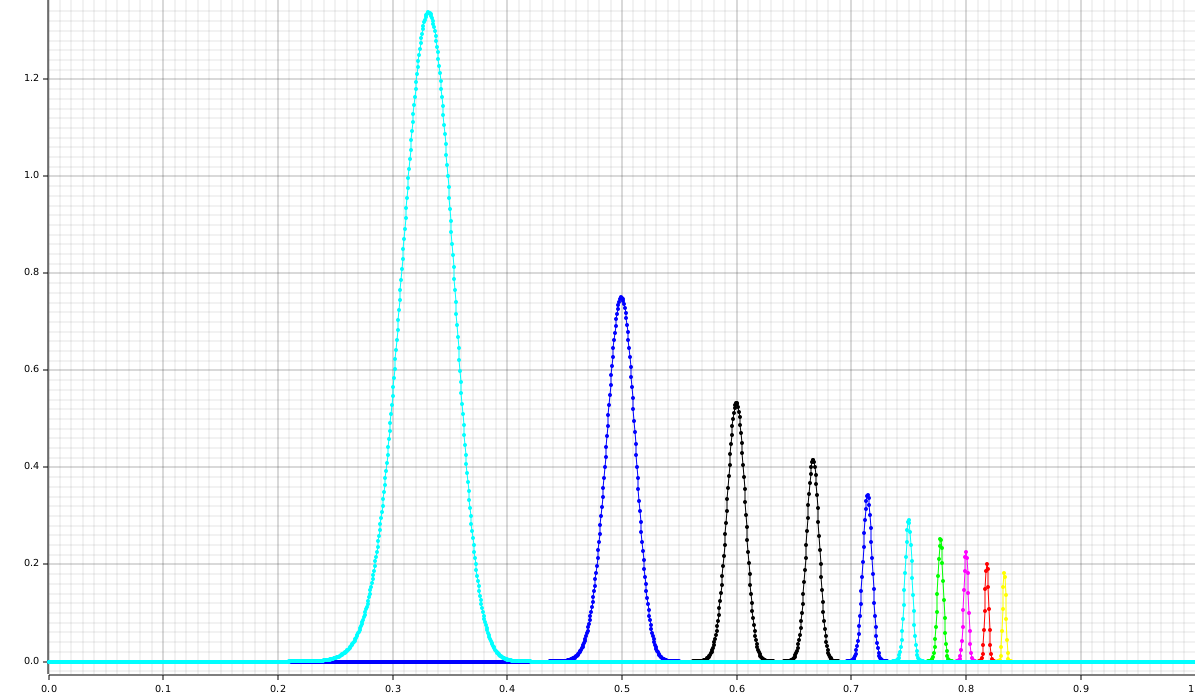
\includegraphics[width=\textwidth]{Images/Incoming_IC.png}
    \end{subfigure}
    \hfill
    \begin{subfigure}[b]{0.43\textwidth}
        \centering
        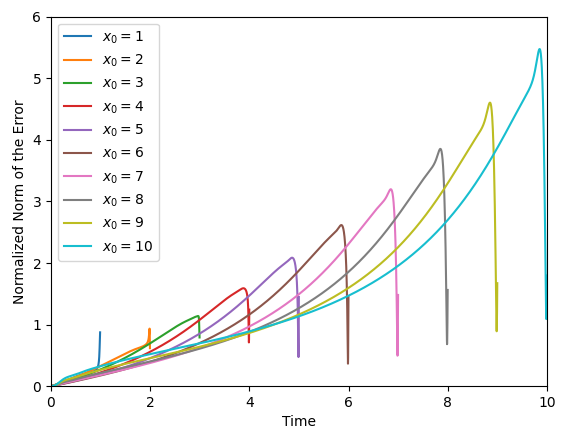
\includegraphics[width=\textwidth]{Images/Incoming_Error.png}
    \end{subfigure}
    \caption{Initial conditions for $\psi$ (left) and the variation in time of the norm of the exact error normalized to the norm of the solution (right).}
    \label{fig:Incoming_Waves}
\end{figure}

We can see just by the initial conditions that incoming waves become more difficult to resolve the further away they are, as the Gaussian gets thinner the closer it is to $\mathscr{I}$. Additionally, we can see that the error increases very rapidly as the waves propagate. Both these results were what we would expect to happen for this coordinate system. Therefore, if we expect incoming waves on our system, we should modify the coordinates to have a traditional Cauchy slice for part of the domain and then join that slice to a hyperboloidal slice when we don't expect to have incoming waves anymore.